\Exhibit{PubScoring}{%
    A help page on pub.dev explaining the scoring of the packages%
}

This page shows that:

\begin{itemize}

    \item \Quote{Likes offer a measure of how many developers have liked a package}.

    \item \Quote{%
        Popularity measures the number of apps that depend on a package over the past 60 days.
        We show this as a percentile from 100\% (among the top 1\% most used packages)
        to 0\% (the least used package).%
    }
\end{itemize}

This means that the popularity percentile and not the like count
is the proper metric to compare how packages are really used.

\begin{center}
    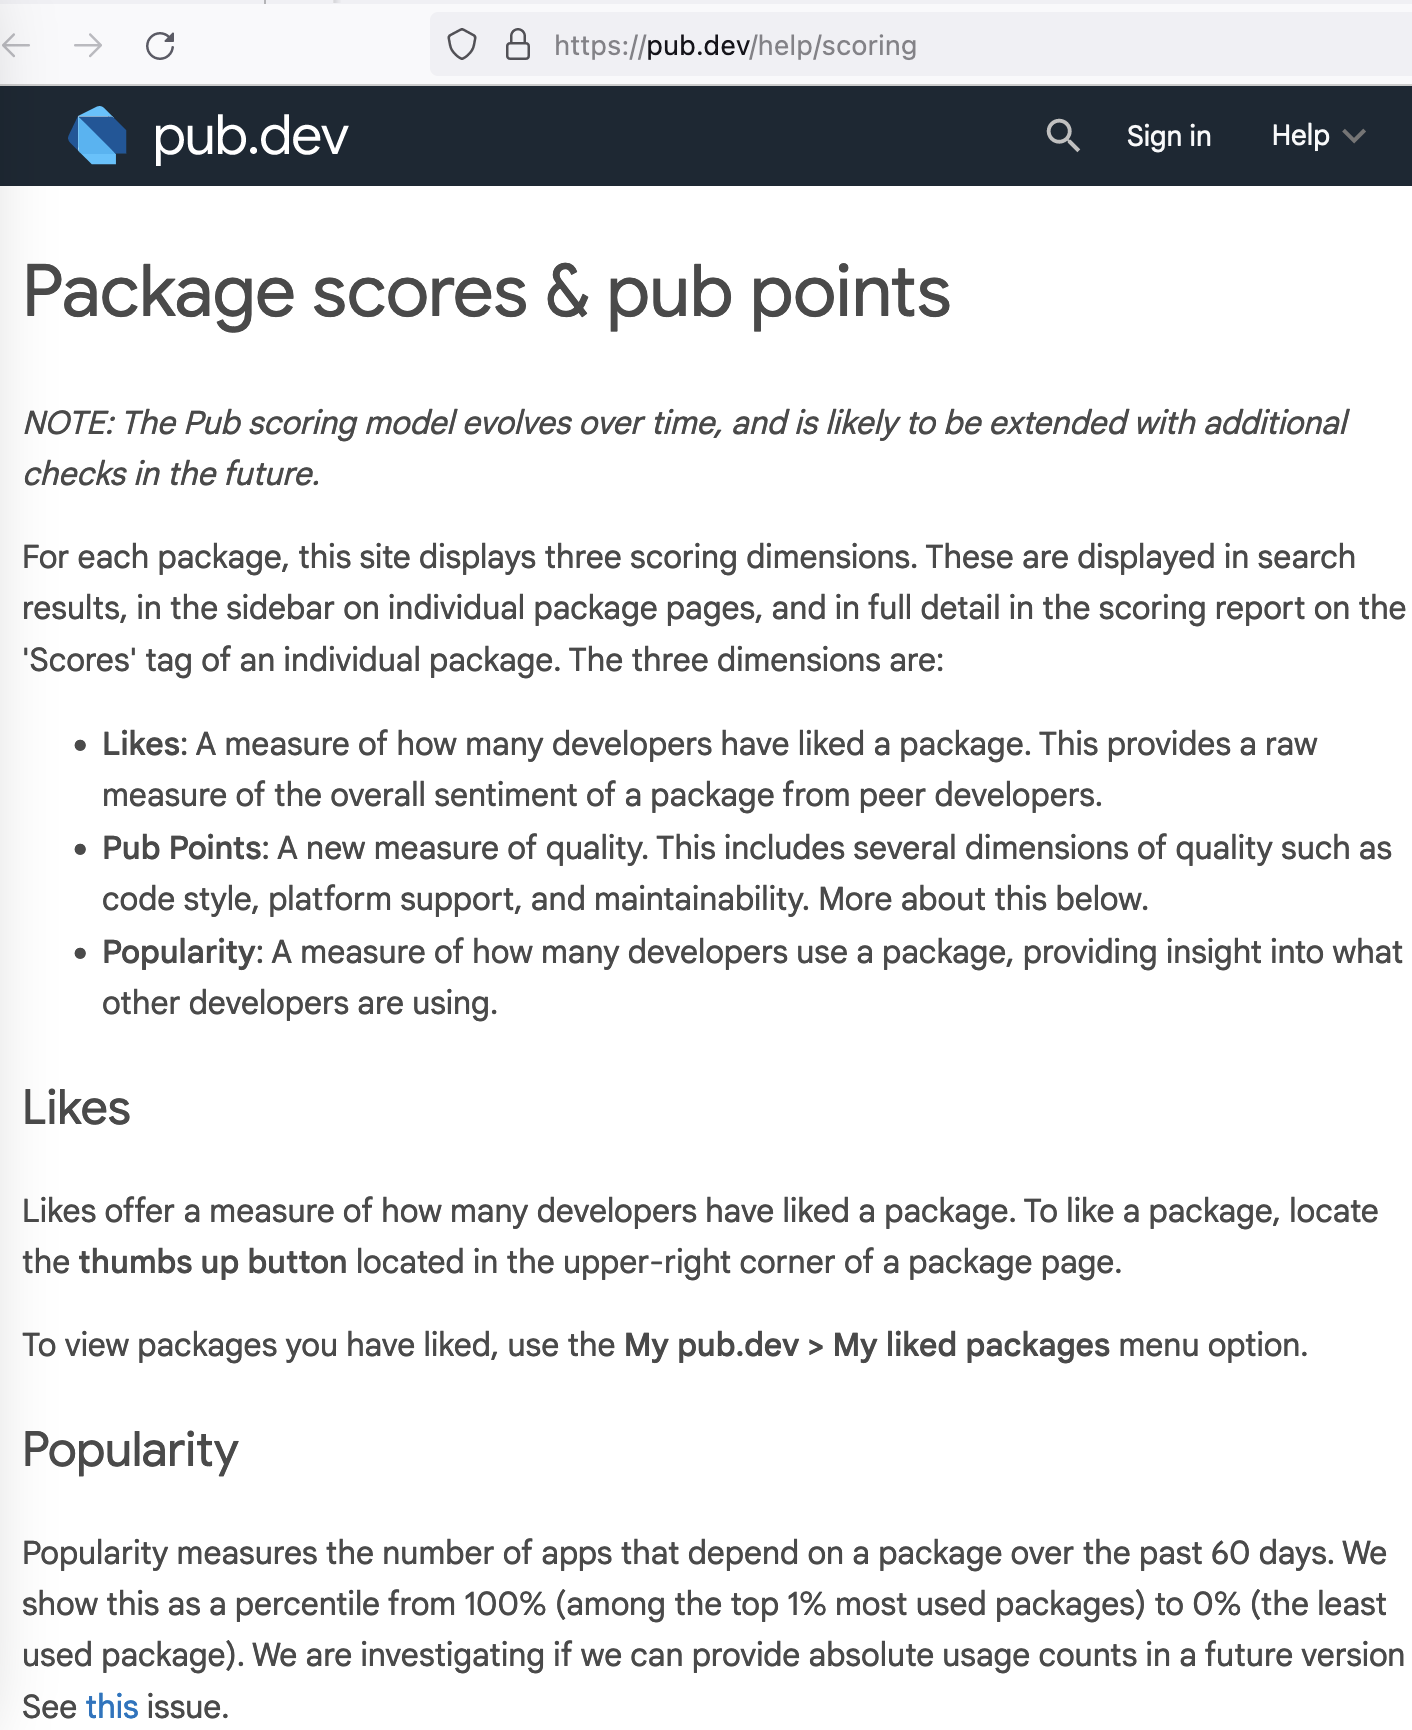
\includegraphics[width=30em]{pub-scoring}
\end{center}

\pagebreak
